\documentclass[11pt,oneside]{book}

\usepackage[margin=1in]{geometry}
\usepackage[T1]{fontenc}
\usepackage[utf8]{inputenc}
\usepackage{lmodern}
\usepackage{microtype}
\usepackage{amsmath,amssymb,amsthm,mathtools,bm}
\usepackage{booktabs,array,tabularx}
\usepackage{enumitem}
\usepackage{float}
\usepackage{caption}
\usepackage{xcolor}
\usepackage{hyperref}
\usepackage[most]{tcolorbox}
\usepackage{tikz}
\usepackage{tikz-3dplot}
\usepackage{pgfplots}
\usepackage{fancyhdr}
\usepackage{titlesec}

\pgfplotsset{compat=1.18}
\usetikzlibrary{arrows.meta,calc,positioning,decorations.pathreplacing,patterns,backgrounds,fit,intersections,shadings}

\definecolor{chapterblue}{HTML}{1F5AA6}
\definecolor{chapterteal}{HTML}{168A8F}
\definecolor{chapterorange}{HTML}{D9822B}
\definecolor{chaptergreen}{HTML}{2D8A4E}
\definecolor{chapterpurple}{HTML}{6B4EAA}
\definecolor{chapterred}{HTML}{B23B3B}
\definecolor{softblue}{HTML}{EAF3FF}
\definecolor{softgreen}{HTML}{EAF8EF}
\definecolor{softorange}{HTML}{FFF4E6}
\definecolor{softpurple}{HTML}{F3EEFF}
\definecolor{softred}{HTML}{FFF0F0}
\definecolor{softgray}{HTML}{F6F7F9}
\definecolor{darkgray}{HTML}{30343B}

\hypersetup{
  colorlinks=true,
  linkcolor=chapterblue,
  urlcolor=chapterblue,
  citecolor=chapterblue,
  pdftitle={Chapter 20. Line Integrals and Work}
}

\setlength{\parindent}{0pt}
\setlength{\parskip}{0.62em}
\setlength{\headheight}{14pt}
\setlist[itemize]{topsep=2pt,itemsep=2pt}
\setlist[enumerate]{topsep=2pt,itemsep=2pt}

\pagestyle{fancy}
\fancyhf{}
\lhead{Chapter 20. Line Integrals and Work}
\rhead{\thepage}
\renewcommand{\headrulewidth}{0.4pt}

\titleformat{\chapter}[display]
  {\normalfont\huge\bfseries\color{chapterblue}}
  {\chaptertitlename\ \thechapter}{8pt}{\Huge}
\titlespacing*{\chapter}{0pt}{-18pt}{20pt}
\titleformat{\section}{\Large\bfseries\color{chapterblue}}{\thesection}{0.6em}{}
\titleformat{\subsection}{\large\bfseries\color{chapterteal}}{\thesubsection}{0.6em}{}

\newcommand{\R}{\mathbb R}
\newcommand{\dd}{\,d}
\newcommand{\vect}[1]{\mathbf{#1}}
\newcommand{\norm}[1]{\left\lVert #1\right\rVert}
\newcommand{\abs}[1]{\left\lvert #1\right\rvert}
\newcommand{\grad}{\nabla}

\tikzset{
  axisline/.style={darkgray, -Latex, line width=0.8pt},
  vector/.style={chapterblue, -Latex, line width=1.3pt},
  vectorred/.style={chapterred, -Latex, line width=1.3pt},
  vectororange/.style={chapterorange, -Latex, line width=1.3pt},
  vectorgreen/.style={chaptergreen, -Latex, line width=1.3pt},
  guide/.style={darkgray!45, dashed, line width=0.6pt},
  point/.style={circle, fill=chapterblue, inner sep=1.7pt},
  redpoint/.style={circle, fill=chapterred, inner sep=1.7pt},
  labelnode/.style={fill=white, inner sep=1pt, font=\small},
  boxnode/.style={draw=chapterblue!60!black, fill=softblue, rounded corners=2pt, align=center, inner sep=5pt},
  greennode/.style={draw=chaptergreen!60!black, fill=softgreen, rounded corners=2pt, align=center, inner sep=5pt},
  orangenode/.style={draw=chapterorange!75!black, fill=softorange, rounded corners=2pt, align=center, inner sep=5pt},
  purplenode/.style={draw=chapterpurple!65!black, fill=softpurple, rounded corners=2pt, align=center, inner sep=5pt},
  rednode/.style={draw=chapterred!65!black, fill=softred, rounded corners=2pt, align=center, inner sep=5pt}
}

\newtcolorbox{mainideabox}[1][]{
  enhanced, breakable,
  colback=softblue, colframe=chapterblue,
  title=\textbf{#1}, fonttitle=\bfseries,
  boxrule=0.8pt, arc=2mm,
  left=2mm,right=2mm,top=1mm,bottom=1mm
}
\newtcolorbox{definitionbox}[1][]{
  enhanced, breakable,
  colback=softgreen, colframe=chaptergreen,
  title=\textbf{#1}, fonttitle=\bfseries,
  boxrule=0.8pt, arc=2mm,
  left=2mm,right=2mm,top=1mm,bottom=1mm
}
\newtcolorbox{examplebox}[1][]{
  enhanced, breakable,
  colback=white, colframe=chapterblue!75!black,
  title=\textbf{#1}, fonttitle=\bfseries,
  boxrule=0.8pt, arc=2mm,
  left=2mm,right=2mm,top=1mm,bottom=1mm
}
\newtcolorbox{warningbox}[1][]{
  enhanced, breakable,
  colback=softorange, colframe=chapterorange,
  title=\textbf{#1}, fonttitle=\bfseries,
  boxrule=0.8pt, arc=2mm,
  left=2mm,right=2mm,top=1mm,bottom=1mm
}
\newtcolorbox{bridgebox}[1][]{
  enhanced, breakable,
  colback=softpurple, colframe=chapterpurple,
  title=\textbf{#1}, fonttitle=\bfseries,
  boxrule=0.8pt, arc=2mm,
  left=2mm,right=2mm,top=1mm,bottom=1mm
}

\begin{document}
\setcounter{chapter}{19}
\chapter{Line Integrals and Work}
\vspace{-1.5em}
{\large\color{darkgray}Accumulating scalar quantities and vector forces along curves}

\section*{Chapter overview}

A definite integral accumulates a quantity along an interval. A double integral accumulates a quantity over a region. A triple integral accumulates a quantity through a solid. A \textbf{line integral} accumulates a quantity along a curve.

Line integrals are the first place where the geometry of a path becomes part of the integral. A curve can bend, twist, move through changing density, or pass through a force field whose direction changes from point to point. The value of the integral may depend not only on the endpoints, but also on the route taken between them.

This chapter develops two closely related ideas:
\begin{enumerate}
  \item \textbf{Scalar line integrals}, written $\int_C f\,ds$, which accumulate a scalar field along a curve.
  \item \textbf{Vector line integrals}, written $\int_C F\cdot dr$, which measure the work done by a vector field along an oriented curve.
\end{enumerate}
The second kind is one of the central objects of vector calculus. It connects geometry, physics, conservative fields, Green's theorem, Stokes' theorem, and the dynamics of optimization algorithms.

\begin{mainideabox}[The main idea]
A line integral is a limit of small contributions along a curve. A curve is chopped into short pieces. On each piece, the field is approximately constant and the curve is approximately straight. The line integral is the limiting sum of all these small contributions.
\end{mainideabox}

\subsection*{Learning goals}
After studying this chapter, you should be able to:
\begin{enumerate}
  \item define and compute scalar line integrals with respect to arc length;
  \item compute line integrals with respect to $x$, $y$, and $z$;
  \item compute vector line integrals using a parameterization of the curve;
  \item interpret $\int_C F\cdot dr$ as work done by a force field;
  \item understand orientation, path dependence, and additivity over piecewise curves;
  \item approximate line integrals numerically from sampled points;
  \item connect line integrals to motion, optimization paths, probability flows, and machine-learning loss landscapes.
\end{enumerate}

\begin{figure}[H]
\centering
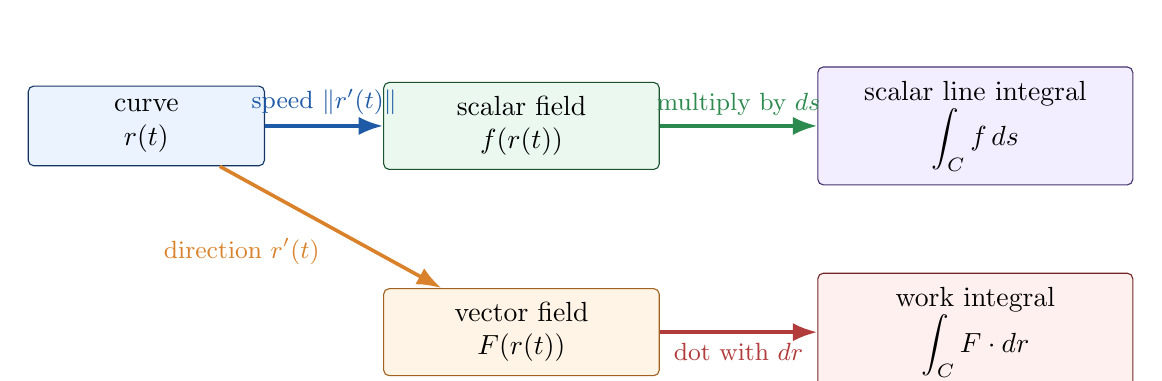
\begin{tikzpicture}[node distance=1.5cm]
  \node[boxnode, minimum width=3.0cm] (curve) {curve\\$r(t)$};
  \node[greennode, right=of curve, minimum width=3.5cm] (scalar) {scalar field\\$f(r(t))$};
  \node[orangenode, below=of scalar, minimum width=3.5cm] (vectorfield) {vector field\\$F(r(t))$};
  \node[purplenode, right=2.0cm of scalar, minimum width=4.0cm] (scalarint) {scalar line integral\\$\displaystyle \int_C f\,ds$};
  \node[rednode, right=2.0cm of vectorfield, minimum width=4.0cm] (work) {work integral\\$\displaystyle \int_C F\cdot dr$};
  \draw[vector] (curve) -- node[above,font=\small] {speed $\norm{r'(t)}$} (scalar);
  \draw[vectororange] (curve) -- node[below left,font=\small] {direction $r'(t)$} (vectorfield);
  \draw[vectorgreen] (scalar) -- node[above,font=\small] {multiply by $ds$} (scalarint);
  \draw[vectorred] (vectorfield) -- node[below,font=\small] {dot with $dr$} (work);
\end{tikzpicture}
\caption{Two line integrals use the same path but accumulate different local quantities. Scalar line integrals use length; vector line integrals use oriented displacement.}
\end{figure}

\section{Oriented curves and parameterizations}

A curve $C$ in the plane or space is usually described by a vector-valued function
\[
r(t)=\langle x(t),y(t)\rangle,\qquad a\le t\le b,
\]
or
\[
r(t)=\langle x(t),y(t),z(t)\rangle,\qquad a\le t\le b.
\]
The direction in which $t$ increases gives the \textbf{orientation} of the curve. The same geometric curve can have the opposite orientation if we traverse it in reverse.

The velocity vector is $r'(t)=\langle x'(t),y'(t)\rangle$ in the plane, or $r'(t)=\langle x'(t),y'(t),z'(t)\rangle$ in space. Its magnitude is the speed along the curve. The arc length differential is
\[
ds=\norm{r'(t)}\,dt.
\]
For a space curve,
\[
\norm{r'(t)}=\sqrt{[x'(t)]^2+[y'(t)]^2+[z'(t)]^2}.
\]

\begin{figure}[H]
\centering
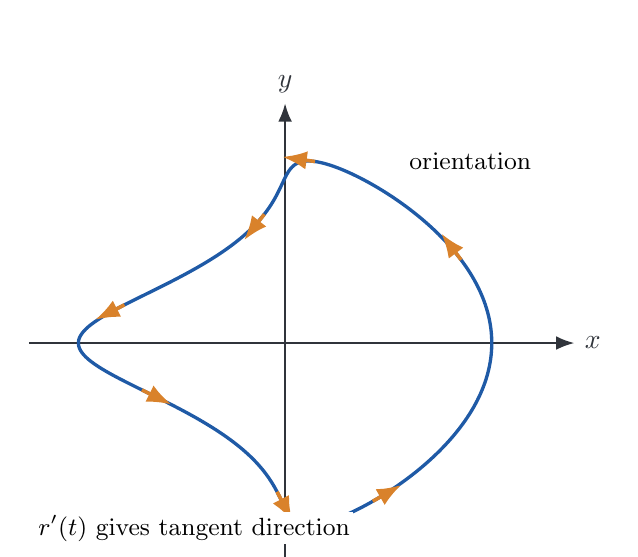
\begin{tikzpicture}[scale=2.1]
  \draw[axisline] (-1.55,0) -- (1.75,0) node[right] {$x$};
  \draw[axisline] (0,-1.35) -- (0,1.45) node[above] {$y$};
  \draw[very thick,chapterblue,domain=0:360,samples=240,smooth,variable=\t]
    plot ({cos(\t)+0.25*cos(3*\t)},{sin(\t)+0.25*sin(2*\t)});
  \foreach \s in {20,65,110,155,210,260,315}{
    \pgfmathsetmacro{\xs}{cos(\s)+0.25*cos(3*\s)}
    \pgfmathsetmacro{\ys}{sin(\s)+0.25*sin(2*\s)}
    \pgfmathsetmacro{\dxs}{-sin(\s)-0.75*sin(3*\s)}
    \pgfmathsetmacro{\dys}{cos(\s)+0.50*cos(2*\s)}
    \pgfmathsetmacro{\len}{sqrt(\dxs*\dxs+\dys*\dys)}
    \draw[vectororange] (\xs,\ys) -- ({\xs+0.20*\dxs/\len},{\ys+0.20*\dys/\len});
  }
  \node[labelnode] at (1.12,1.10) {orientation};
  \node[labelnode] at (-0.55,-1.12) {$r'(t)$ gives tangent direction};
\end{tikzpicture}
\caption{An oriented curve with tangent vectors. The arrows show the direction in which the parameter increases.}
\end{figure}

\section{Scalar line integrals with respect to arc length}

Suppose $f(x,y)$ is a scalar field defined on a curve $C$. The scalar line integral of $f$ along $C$ with respect to arc length is
\[
\int_C f(x,y)\,ds.
\]
If $C$ is parameterized by $r(t)=\langle x(t),y(t)\rangle$ for $a\le t\le b$, then
\[
\int_C f(x,y)\,ds
=
\int_a^b f(x(t),y(t))\sqrt{[x'(t)]^2+[y'(t)]^2}\,dt.
\]
For a space curve $r(t)=\langle x(t),y(t),z(t)\rangle$,
\[
\int_C f(x,y,z)\,ds
=
\int_a^b f(x(t),y(t),z(t))\sqrt{[x'(t)]^2+[y'(t)]^2+[z'(t)]^2}\,dt.
\]
The factor $ds=\norm{r'(t)}dt$ converts the parameter interval into actual distance traveled along the curve.

\begin{definitionbox}[Scalar line integrals do not depend on orientation]
Because $ds$ measures length, reversing the orientation of the same curve does not change $\int_C f\,ds$. The curve is traversed in the opposite direction, but the same small lengths are added.
\end{definitionbox}

\begin{examplebox}[Example 1: scalar line integral over a quarter circle]
Evaluate
\[
\int_C (3-xy^2)\,ds,
\]
where $C$ is the first-quadrant part of the unit circle $x^2+y^2=1$.
Use
\[
r(t)=\langle \cos t,\sin t\rangle,\qquad 0\le t\le \frac{\pi}{2}.
\]
Then
\[
r'(t)=\langle -\sin t,\cos t\rangle,\qquad \norm{r'(t)}=1.
\]
Therefore
\[
\begin{aligned}
\int_C (3-xy^2)\,ds
&=\int_0^{\pi/2}\left(3-\cos t\sin^2t\right)\,dt\\
&=\frac{3\pi}{2}-\frac13.
\end{aligned}
\]
\end{examplebox}

\begin{figure}[H]
\centering
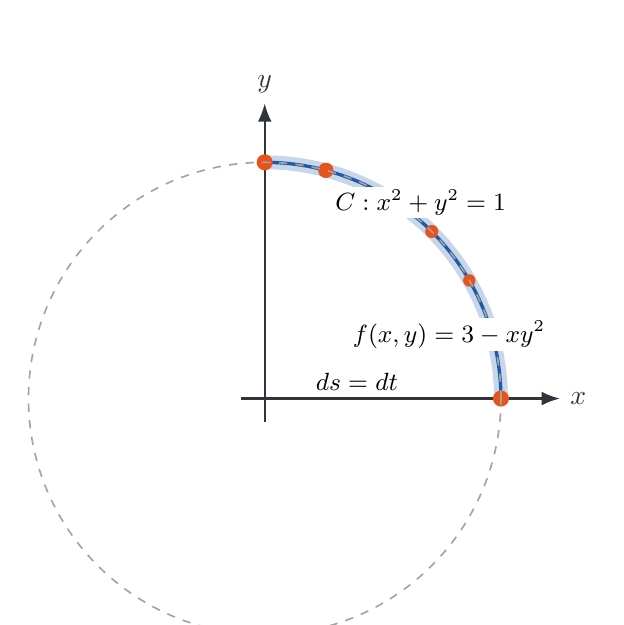
\begin{tikzpicture}[scale=3.0]
  \draw[axisline] (-0.1,0) -- (1.25,0) node[right] {$x$};
  \draw[axisline] (0,-0.1) -- (0,1.25) node[above] {$y$};
  \draw[chapterblue!25, line width=5pt, domain=0:90, samples=120] plot ({cos(\x)},{sin(\x)});
  \draw[chapterblue, very thick, domain=0:90, samples=120] plot ({cos(\x)},{sin(\x)});
  \foreach \ang/\val in {0/3.00,15/2.75,30/2.57,45/2.65,60/2.78,75/2.92,90/3.00}{
    \pgfmathsetmacro{\xx}{cos(\ang)}
    \pgfmathsetmacro{\yy}{sin(\ang)}
    \pgfmathsetmacro{\rad}{0.025+0.018*(\val-2.5)}
    \fill[chapterorange!65!red] (\xx,\yy) circle (\rad);
  }
  \draw[guide] (0,0) circle (1);
  \node[labelnode] at (0.66,0.83) {$C: x^2+y^2=1$};
  \node[labelnode] at (0.78,0.27) {$f(x,y)=3-xy^2$};
  \node[labelnode] at (0.39,0.07) {$ds=dt$};
\end{tikzpicture}
\caption{A scalar field sampled along a quarter circle. A scalar line integral accumulates field values weighted by arc length. Larger dots indicate larger sampled field values.}
\end{figure}

\section{Mass of a wire}

A major interpretation of a scalar line integral is the mass of a thin wire. Suppose a wire has shape $C$ and density $\rho(x,y,z)$ measured in mass per unit length. Then the mass is
\[
M=\int_C \rho(x,y,z)\,ds.
\]
If the density is constant, this becomes density times length. If the density changes from point to point, the line integral accumulates the varying density along the wire.

\begin{examplebox}[Example 2: mass of a helical wire]
Let $C$ be the helix
\[
r(t)=\langle \sin t,\cos t,t\rangle,\qquad 0\le t\le \pi.
\]
Suppose the density is $\rho(x,y,z)=2x\sin z$. Then $\rho(r(t))=2\sin^2t$. Also
\[
r'(t)=\langle \cos t,-\sin t,1\rangle,\qquad \norm{r'(t)}=\sqrt2.
\]
Thus
\[
\int_C 2x\sin z\,ds
=
\int_0^\pi 2\sin^2t\sqrt2\,dt
=
\pi\sqrt2.
\]
\end{examplebox}

\begin{figure}[H]
\centering
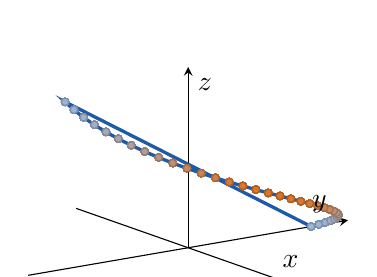
\begin{tikzpicture}
\begin{axis}[
  width=0.70\textwidth,
  height=0.46\textwidth,
  view={55}{28},
  axis lines=center,
  xlabel={$x$}, ylabel={$y$}, zlabel={$z$},
  xmin=-1.3,xmax=1.3,ymin=-1.3,ymax=1.3,zmin=0,zmax=3.4,
  ticks=none,
  colormap={density}{color=(chapterblue!45) color=(chapterorange!90!red)}
]
\addplot3[domain=0:180,samples=90,very thick,chapterblue] ({sin(x)},{cos(x)},{x*pi/180});
\addplot3[scatter,only marks,mark=*,mark size=1.3pt,domain=0:180,samples=34,
  scatter src={sin(x)^2}] ({sin(x)},{cos(x)},{x*pi/180});
\end{axis}
\end{tikzpicture}
\caption{A helix with scalar density sampled along the curve. The scalar line integral gives the mass of a wire with this density.}
\end{figure}

\section{Line integrals with respect to coordinates}

Line integrals can also be taken with respect to coordinates. In the plane, we may see
\[
\int_C f(x,y)\,dx,\qquad \int_C g(x,y)\,dy.
\]
If $C$ is parameterized by $x=x(t)$ and $y=y(t)$, then
\[
\int_C f(x,y)\,dx=\int_a^b f(x(t),y(t))x'(t)\,dt,
\]
and
\[
\int_C g(x,y)\,dy=\int_a^b g(x(t),y(t))y'(t)\,dt.
\]
In space, similarly,
\[
\int_C f(x,y,z)\,dz=\int_a^b f(x(t),y(t),z(t))z'(t)\,dt.
\]
Unlike $ds$, the coordinate differentials $dx$, $dy$, and $dz$ can be positive or negative. Therefore coordinate line integrals depend on orientation.

\begin{warningbox}[$ds$ versus $dx$, $dy$, and $dz$]
The symbol $ds$ is a length element and is always nonnegative. The symbols $dx$, $dy$, and $dz$ are signed coordinate changes. Reversing the orientation of a curve leaves $\int_C f\,ds$ unchanged, but changes the sign of $\int_C f\,dx$, $\int_C f\,dy$, and $\int_C f\,dz$.
\end{warningbox}

\begin{figure}[H]
\centering
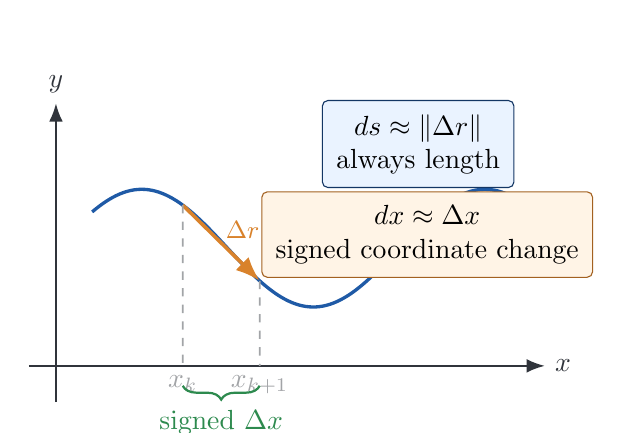
\begin{tikzpicture}[scale=1.15]
  \draw[axisline] (-0.3,0) -- (5.4,0) node[right] {$x$};
  \draw[axisline] (0,-0.4) -- (0,2.9) node[above] {$y$};
  \draw[very thick,chapterblue,domain=0.4:5.0,samples=120] plot (\x,{1.3+0.65*sin(95*\x)});
  \coordinate (A) at (1.4,{1.3+0.65*sin(95*1.4)});
  \coordinate (B) at (2.25,{1.3+0.65*sin(95*2.25)});
  \draw[vectororange] (A) -- (B) node[midway,above right,labelnode] {$\Delta r$};
  \draw[guide] (A) -- (1.4,0) node[below] {$x_k$};
  \draw[guide] (B) -- (2.25,0) node[below] {$x_{k+1}$};
  \draw[decorate,decoration={brace,mirror,amplitude=5pt},chaptergreen,thick] (1.4,-0.22) -- (2.25,-0.22)
    node[midway,below=5pt] {signed $\Delta x$};
  \node[boxnode] at (4.0,2.45) {$ds\approx \norm{\Delta r}$\\always length};
  \node[orangenode] at (4.1,1.45) {$dx\approx \Delta x$\\signed coordinate change};
\end{tikzpicture}
\caption{The arc length element $ds$ measures actual distance along the curve, while $dx$ measures signed horizontal change.}
\end{figure}

\section{Vector line integrals and work}

Suppose an object is displaced by a vector $d$ while a constant force $F$ acts on it. The work done is
\[
W=F\cdot d.
\]
If the force varies from point to point and the object moves along a curve $C$, we chop the curve into small displacement vectors $\Delta r$. On each small piece, the work is approximately $F\cdot \Delta r$. Adding these contributions and taking a limit gives the vector line integral
\[
\int_C F\cdot dr.
\]
If $F(x,y)=\langle P(x,y),Q(x,y)\rangle$ and $r(t)=\langle x(t),y(t)\rangle$, then
\[
\int_C F\cdot dr=\int_a^b F(r(t))\cdot r'(t)\,dt.
\]
Equivalently,
\[
\int_C F\cdot dr=\int_C P\,dx+Q\,dy.
\]
In space, if $F(x,y,z)=\langle P,Q,R\rangle$, then
\[
\int_C F\cdot dr=\int_C P\,dx+Q\,dy+R\,dz.
\]

\begin{mainideabox}[The computation recipe]
To compute $\int_C F\cdot dr$:
\begin{enumerate}
  \item parameterize the curve as $r(t)$;
  \item compute $r'(t)$;
  \item substitute the parameterization into the field to get $F(r(t))$;
  \item take the dot product $F(r(t))\cdot r'(t)$;
  \item integrate with respect to $t$ over the parameter interval.
\end{enumerate}
\end{mainideabox}

\begin{figure}[H]
\centering
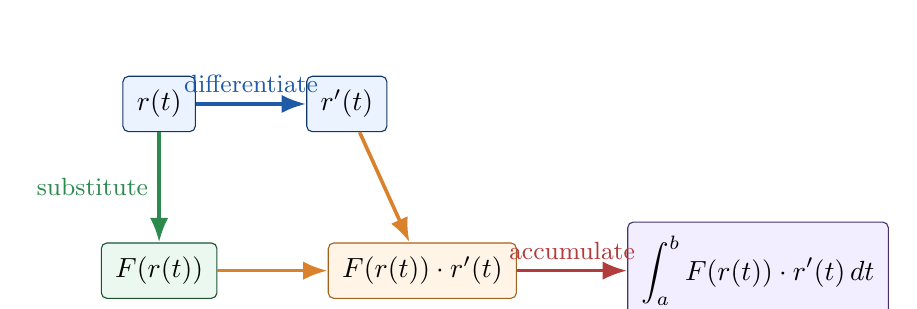
\begin{tikzpicture}[node distance=1.4cm]
  \node[boxnode] (param) {$r(t)$};
  \node[boxnode, right=of param] (vel) {$r'(t)$};
  \node[greennode, below=of param] (field) {$F(r(t))$};
  \node[orangenode, right=of field] (dot) {$F(r(t))\cdot r'(t)$};
  \node[purplenode, right=of dot] (int) {$\displaystyle \int_a^b F(r(t))\cdot r'(t)\,dt$};
  \draw[vector] (param) -- node[above,font=\small] {differentiate} (vel);
  \draw[vectorgreen] (param) -- node[left,font=\small] {substitute} (field);
  \draw[vectororange] (vel) -- (dot);
  \draw[vectororange] (field) -- (dot);
  \draw[vectorred] (dot) -- node[above,font=\small] {accumulate} (int);
\end{tikzpicture}
\caption{The standard workflow for a vector line integral.}
\end{figure}

\begin{examplebox}[Example 3: work along a circular arc]
Let
\[
F(x,y)=\langle y^2,-xy\rangle,
\]
and let $C$ be the curve
\[
r(t)=\langle \sin t,\cos t\rangle,\qquad 0\le t\le \frac{\pi}{2}.
\]
Then $r'(t)=\langle \cos t,-\sin t\rangle$. Substituting into the vector field gives
\[
F(r(t))=\langle \cos^2t,-\sin t\cos t\rangle.
\]
The dot product is
\[
F(r(t))\cdot r'(t)=\cos^3t+\sin^2t\cos t=\cos t.
\]
Therefore
\[
\int_C F\cdot dr=\int_0^{\pi/2}\cos t\,dt=1.
\]
\end{examplebox}

\begin{figure}[H]
\centering
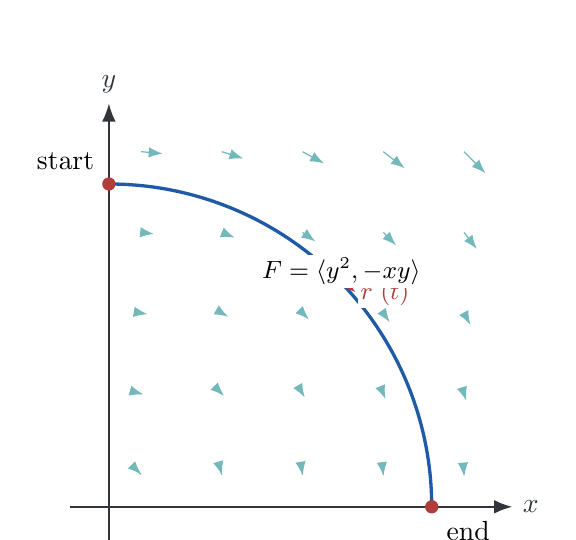
\begin{tikzpicture}[scale=4.1]
  \draw[axisline] (-0.12,0) -- (1.25,0) node[right] {$x$};
  \draw[axisline] (0,-0.12) -- (0,1.25) node[above] {$y$};
  \foreach \xx in {0.1,0.35,0.6,0.85,1.1}{
    \foreach \yy in {0.1,0.35,0.6,0.85,1.1}{
      \pgfmathsetmacro{\uu}{\yy*\yy}
      \pgfmathsetmacro{\vv}{-\xx*\yy}
      \draw[chapterteal!60,-Latex,line width=0.45pt] (\xx,\yy) -- ({\xx+0.055*\uu},{\yy+0.055*\vv});
    }
  }
  \draw[very thick,chapterblue,domain=0:90,samples=120] plot ({sin(\x)},{cos(\x)});
  \draw[vectorred] ({sin(40)},{cos(40)}) -- ++({0.16*cos(40)},{-0.16*sin(40)}) node[right,labelnode] {$r'(t)$};
  \node[redpoint,label=above left:{start}] at (0,1) {};
  \node[redpoint,label=below right:{end}] at (1,0) {};
  \node[labelnode] at (0.72,0.73) {$F=\langle y^2,-xy\rangle$};
\end{tikzpicture}
\caption{Work along a circular arc in a vector field. The integrand is the tangential component of the field times speed.}
\end{figure}

\section{Orientation matters for vector line integrals}

Let $-C$ denote the same curve as $C$ but with the opposite orientation. Then
\[
\int_{-C}F\cdot dr=-\int_C F\cdot dr.
\]
This agrees with the work interpretation. Pushing an object forward along a path may do positive work; moving the same object backward through the same field reverses the displacement direction and reverses the sign of the work.

\begin{examplebox}[Example 4: reversing a path]
For the field and curve in Example 3,
\[
\int_C F\cdot dr=1.
\]
If the same arc is traversed from $(1,0)$ back to $(0,1)$, then
\[
\int_{-C}F\cdot dr=-1.
\]
This sign change is one of the most common sources of mistakes in vector line integrals.
\end{examplebox}

\section{Piecewise smooth curves}

Many useful curves are not given by one formula. They are built from several smooth pieces. If
\[
C=C_1\cup C_2\cup\cdots\cup C_m
\]
with compatible orientations, then
\[
\int_C F\cdot dr=\int_{C_1}F\cdot dr+\int_{C_2}F\cdot dr+\cdots+\int_{C_m}F\cdot dr.
\]
The same additivity holds for scalar line integrals.

\begin{examplebox}[Example 5: a piecewise line integral in space]
Evaluate
\[
\int_C y\,dx+z\,dy+x\,dz,
\]
where $C=C_1\cup C_2$, $C_1$ is the line segment from $(3,4,0)$ to $(3,4,5)$, and $C_2$ is the line segment from $(3,4,5)$ to $(2,0,0)$.

For $C_1$, use $r_1(t)=\langle 3,4,t\rangle$, $0\le t\le 5$. Then $dx=0$, $dy=0$, and $dz=dt$, so
\[
\int_{C_1} y\,dx+z\,dy+x\,dz=\int_0^5 3\,dt=15.
\]
For $C_2$, use $r_2(s)=\langle 3-s,4-4s,5-5s\rangle$, $0\le s\le 1$. Then $dx=-ds$, $dy=-4ds$, and $dz=-5ds$. Therefore
\[
\begin{aligned}
\int_{C_2} y\,dx+z\,dy+x\,dz
&=\int_0^1\left[(4-4s)(-1)+(5-5s)(-4)+(3-s)(-5)\right]ds\\
&=\int_0^1(-39+29s)\,ds=-\frac{49}{2}.
\end{aligned}
\]
Thus
\[
\int_C y\,dx+z\,dy+x\,dz=15-\frac{49}{2}=-\frac{19}{2}.
\]
\end{examplebox}

\begin{figure}[H]
\centering
\tdplotsetmaincoords{68}{116}
\begin{tikzpicture}[tdplot_main_coords,scale=0.95]
  \draw[axisline] (0,0,0) -- (4.2,0,0) node[anchor=north east] {$x$};
  \draw[axisline] (0,0,0) -- (0,4.8,0) node[anchor=north west] {$y$};
  \draw[axisline] (0,0,0) -- (0,0,5.8) node[anchor=south] {$z$};
  \coordinate (A) at (3,4,0);
  \coordinate (B) at (3,4,5);
  \coordinate (C) at (2,0,0);
  \draw[very thick,chapterblue,-Latex] (A) -- (B);
  \draw[very thick,chapterred,-Latex] (B) -- (C);
  \fill[chapterblue] (A) circle (2pt) node[below right] {$(3,4,0)$};
  \fill[chapterorange] (B) circle (2pt) node[above right] {$(3,4,5)$};
  \fill[chapterred] (C) circle (2pt) node[below] {$(2,0,0)$};
  \draw[guide] (3,4,0) -- (3,0,0) -- (0,0,0);
  \node[labelnode] at (2.2,4.2,2.8) {$C_1$};
  \node[labelnode] at (2.5,1.9,2.5) {$C_2$};
\end{tikzpicture}
\caption{A piecewise curve in space. Line integrals over piecewise curves are computed one segment at a time.}
\end{figure}

\section{Path dependence}

A major difference between line integrals and ordinary definite integrals is that path matters. Two different curves with the same starting and ending points can produce different line integrals.

\begin{examplebox}[Example 6: same endpoints, different paths]
Let $F(x,y)=\langle y,0\rangle$. We compute the work from $(0,0)$ to $(1,1)$ along two paths.

\textbf{Path A: straight line.} Let $r_A(t)=\langle t,t\rangle$, $0\le t\le 1$. Then $F(r_A(t))=\langle t,0\rangle$ and $r_A'(t)=\langle 1,1\rangle$. Therefore
\[
\int_{C_A}F\cdot dr=\int_0^1 t\,dt=\frac12.
\]

\textbf{Path B: horizontal then vertical.} First go from $(0,0)$ to $(1,0)$, then from $(1,0)$ to $(1,1)$. On the horizontal segment, $y=0$, so $F=\langle 0,0\rangle$. On the vertical segment, $dx=0$, and $F\cdot dr=y\,dx=0$. Hence
\[
\int_{C_B}F\cdot dr=0.
\]
The endpoints are the same, but the work is different. This field is path-dependent.
\end{examplebox}

\begin{figure}[H]
\centering
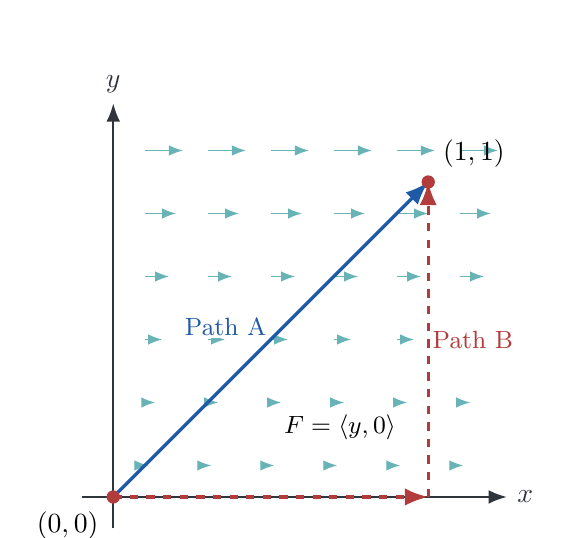
\begin{tikzpicture}[scale=4.0]
  \draw[axisline] (-0.1,0) -- (1.25,0) node[right] {$x$};
  \draw[axisline] (0,-0.1) -- (0,1.25) node[above] {$y$};
  \foreach \xx in {0.1,0.3,0.5,0.7,0.9,1.1}{
    \foreach \yy in {0.1,0.3,0.5,0.7,0.9,1.1}{
      \draw[chapterteal!65,-Latex,line width=0.45pt] (\xx,\yy) -- ({\xx+0.11*\yy},{\yy});
    }
  }
  \draw[very thick,chapterblue,-Latex] (0,0) -- (1,1) node[midway,above left,labelnode] {Path A};
  \draw[very thick,chapterred,dashed,-Latex] (0,0) -- (1,0);
  \draw[very thick,chapterred,dashed,-Latex] (1,0) -- (1,1) node[midway,right,labelnode] {Path B};
  \node[redpoint,label=below left:{$(0,0)$}] at (0,0) {};
  \node[redpoint,label=above right:{$(1,1)$}] at (1,1) {};
  \node[labelnode] at (0.72,0.22) {$F=\langle y,0\rangle$};
\end{tikzpicture}
\caption{Two paths with the same endpoints can produce different vector line integrals.}
\end{figure}

\section{A three-dimensional work integral}

Let
\[
F(x,y,z)=\langle xy,yz,zx\rangle
\]
and let $C$ be parameterized by
\[
r(t)=\langle t,t^2,t^3\rangle,\qquad 0\le t\le 1.
\]
Then $r'(t)=\langle 1,2t,3t^2\rangle$. Substituting into $F$ gives
\[
F(r(t))=\langle t^3,t^5,t^4\rangle.
\]
Thus
\[
F(r(t))\cdot r'(t)=t^3+2t^6+3t^6=t^3+5t^6.
\]
Therefore
\[
\int_C F\cdot dr=\int_0^1(t^3+5t^6)\,dt=\frac14+\frac57=\frac{27}{28}.
\]

\begin{figure}[H]
\centering
\tdplotsetmaincoords{70}{112}
\begin{tikzpicture}[tdplot_main_coords,scale=4.2]
  \draw[axisline] (0,0,0) -- (1.25,0,0) node[anchor=north east] {$x$};
  \draw[axisline] (0,0,0) -- (0,1.25,0) node[anchor=north west] {$y$};
  \draw[axisline] (0,0,0) -- (0,0,1.25) node[anchor=south] {$z$};
  \draw[very thick,chapterblue,smooth]
    plot coordinates {(0,0,0) (0.10,0.01,0.001) (0.20,0.04,0.008) (0.30,0.09,0.027) (0.40,0.16,0.064) (0.50,0.25,0.125) (0.60,0.36,0.216) (0.70,0.49,0.343) (0.80,0.64,0.512) (0.90,0.81,0.729) (1.00,1.00,1.00)};
  \foreach \t in {0.18,0.36,0.54,0.72,0.90}{
    \pgfmathsetmacro{\y}{\t*\t}
    \pgfmathsetmacro{\z}{\t*\t*\t}
    \pgfmathsetmacro{\dy}{2*\t}
    \pgfmathsetmacro{\dz}{3*\t*\t}
    \pgfmathsetmacro{\len}{sqrt(1+\dy*\dy+\dz*\dz)}
    \draw[vectororange] (\t,\y,\z) -- ({\t+0.10/\len},{\y+0.10*\dy/\len},{\z+0.10*\dz/\len});
  }
  \fill[chapterred] (0,0,0) circle (0.5pt) node[below] {$t=0$};
  \fill[chapterred] (1,1,1) circle (0.5pt) node[above right] {$t=1$};
  \node[labelnode] at (0.68,0.28,0.70) {$r(t)=\langle t,t^2,t^3\rangle$};
\end{tikzpicture}
\caption{A space curve used for a three-dimensional work integral, with tangent directions shown along the path.}
\end{figure}

\section{Numerical approximation of vector line integrals}

If a curve is sampled at points
\[
r_0,r_1,\ldots,r_N,
\]
then a numerical approximation to the work integral is
\[
\int_C F\cdot dr\approx \sum_{k=0}^{N-1}F\left(\frac{r_k+r_{k+1}}{2}\right)\cdot (r_{k+1}-r_k).
\]
This is the midpoint rule along a curve. It is useful when the curve is known only from data, simulation output, robot trajectories, or numerical solutions of differential equations.

\begin{figure}[H]
\centering
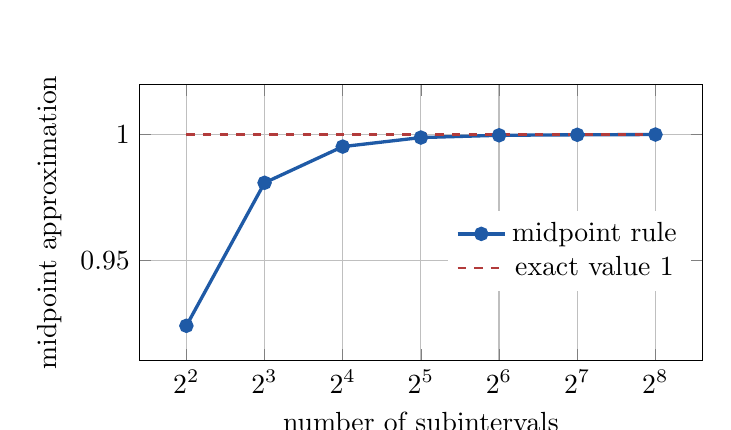
\begin{tikzpicture}
\begin{axis}[
  width=0.72\textwidth,
  height=0.42\textwidth,
  xmode=log,
  log basis x=2,
  xlabel={number of subintervals},
  ylabel={midpoint approximation},
  ymin=0.91,ymax=1.02,
  grid=both,
  legend style={draw=none,fill=white,at={(0.98,0.25)},anchor=south east}
]
\addplot[very thick,chapterblue,mark=*] coordinates {(4,0.9239) (8,0.9808) (16,0.9952) (32,0.9988) (64,0.9997) (128,0.9999) (256,1.0000)};
\addlegendentry{midpoint rule}
\addplot[chapterred,dashed,thick] coordinates {(4,1) (256,1)};
\addlegendentry{exact value $1$}
\end{axis}
\end{tikzpicture}
\caption{Numerical midpoint approximations converge to the vector line integral as the curve sampling becomes finer.}
\end{figure}

\section{Line integrals along optimization paths}

In machine learning and statistics, we often study a loss function $L(\theta)$, where $\theta$ is a vector of parameters. The gradient $\nabla L(\theta)$ is a vector field on parameter space. An optimization algorithm produces a path
\[
\theta_0,\theta_1,\theta_2,\ldots
\]
through that space.

The work-like quantity
\[
\int_C \nabla L\cdot d\theta
\]
measures accumulated change of the loss along the path. For a smooth path, the chain rule gives
\[
\frac{d}{dt}L(\theta(t))=\nabla L(\theta(t))\cdot \theta'(t),
\]
so line integrals of gradients are closely tied to change in objective values. This idea becomes the Fundamental Theorem for Line Integrals in the next chapter.

\begin{figure}[H]
\centering
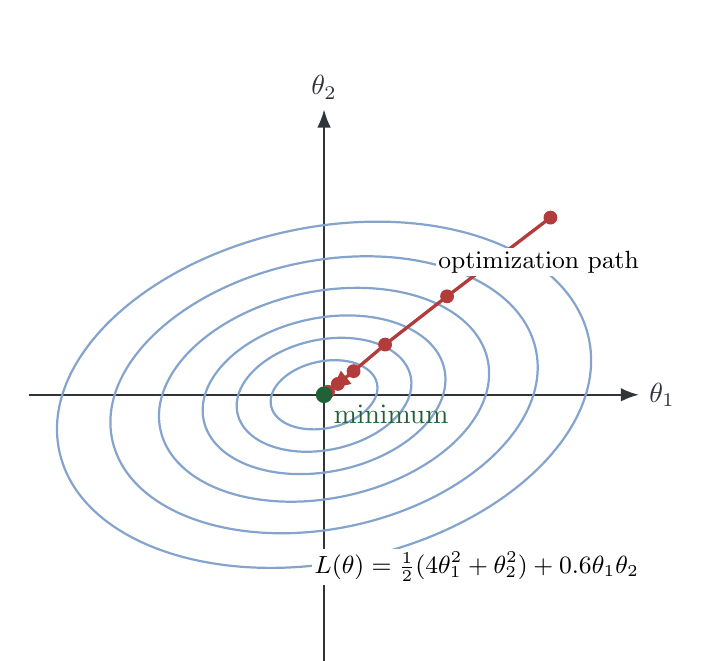
\begin{tikzpicture}[scale=1.25]
  \draw[axisline] (-3,0) -- (3.2,0) node[right] {$\theta_1$};
  \draw[axisline] (0,-2.8) -- (0,2.9) node[above] {$\theta_2$};
  \foreach \a/\b in {0.55/0.34,0.9/0.56,1.25/0.78,1.7/1.05,2.2/1.36,2.75/1.70}{
    \draw[chapterblue!55,thick,rotate=12] (0,0) ellipse ({\a} and {\b});
  }
  \draw[very thick,chapterred,-Latex]
    (2.3,1.8) -- (1.25,1.0) -- (0.62,0.51) -- (0.30,0.24) -- (0.14,0.11) -- (0.04,0.03);
  \foreach \p in {(2.3,1.8),(1.25,1.0),(0.62,0.51),(0.30,0.24),(0.14,0.11),(0.04,0.03)}{
    \fill[chapterred] \p circle (2pt);
  }
  \fill[chaptergreen!70!black] (0,0) circle (2.4pt) node[below right] {minimum};
  \node[labelnode] at (1.55,-1.75) {$L(\theta)=\frac12(4\theta_1^2+\theta_2^2)+0.6\theta_1\theta_2$};
  \node[labelnode] at (2.18,1.35) {optimization path};
\end{tikzpicture}
\caption{A path through a quadratic loss landscape. Line integrals can measure accumulated change along paths in parameter space.}
\end{figure}

\section{Work, circulation, and flow}

The vector line integral $\int_C F\cdot dr$ measures the component of the field tangent to the curve. If the field points mostly along the direction of motion, the integral is positive. If it points mostly opposite the direction of motion, the integral is negative. If the field is mostly perpendicular to the motion, the contribution is small.

For a closed curve, the integral
\[
\oint_C F\cdot dr
\]
is called the \textbf{circulation} of $F$ around $C$. Circulation measures how much the vector field tends to push around the loop. It is a central idea behind Green's theorem and Stokes' theorem.

\begin{examplebox}[Example 7: circulation of a rotational field]
Let $F(x,y)=\langle -y,x\rangle$. On the unit circle with counterclockwise orientation,
\[
r(t)=\langle \cos t,\sin t\rangle,\qquad 0\le t\le 2\pi.
\]
Then
\[
F(r(t))=\langle -\sin t,\cos t\rangle,
\qquad
r'(t)=\langle -\sin t,\cos t\rangle.
\]
Thus $F(r(t))\cdot r'(t)=1$, so
\[
\oint_C F\cdot dr=\int_0^{2\pi}1\,dt=2\pi.
\]
\end{examplebox}

\begin{figure}[H]
\centering
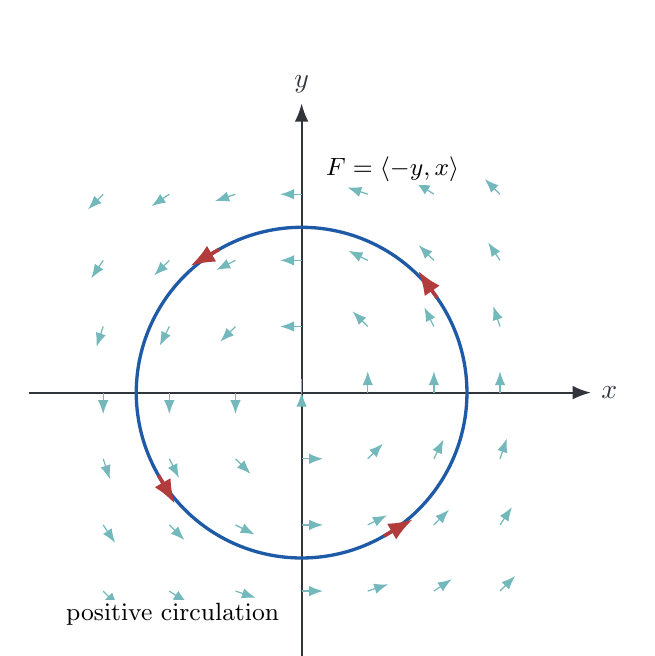
\begin{tikzpicture}[scale=2.1]
  \draw[axisline] (-1.65,0) -- (1.75,0) node[right] {$x$};
  \draw[axisline] (0,-1.65) -- (0,1.75) node[above] {$y$};
  \foreach \xx in {-1.2,-0.8,-0.4,0,0.4,0.8,1.2}{
    \foreach \yy in {-1.2,-0.8,-0.4,0,0.4,0.8,1.2}{
      \pgfmathsetmacro{\uu}{-\yy}
      \pgfmathsetmacro{\vv}{\xx}
      \pgfmathsetmacro{\len}{sqrt(\uu*\uu+\vv*\vv)+0.001}
      \draw[chapterteal!60,-Latex,line width=0.45pt] (\xx,\yy) -- ({\xx+0.13*\uu/\len},{\yy+0.13*\vv/\len});
    }
  }
  \draw[very thick,chapterblue,domain=0:360,samples=240] plot ({cos(\x)},{sin(\x)});
  \foreach \s in {35,120,210,300}{
    \draw[vectorred] ({cos(\s)},{sin(\s)}) -- ({cos(\s)-0.20*sin(\s)},{sin(\s)+0.20*cos(\s)});
  }
  \node[labelnode] at (0.55,1.35) {$F=\langle -y,x\rangle$};
  \node[labelnode] at (-0.78,-1.34) {positive circulation};
\end{tikzpicture}
\caption{Positive circulation around the unit circle for the rotational field $F=\langle -y,x\rangle$.}
\end{figure}

\section{Common mistakes}

\begin{warningbox}[Mistake 1: forgetting $\norm{r'(t)}$ in scalar line integrals]
For scalar line integrals, the formula is
\[
\int_C f\,ds=\int_a^b f(r(t))\norm{r'(t)}\,dt.
\]
The factor $\norm{r'(t)}$ is essential unless the parameterization has unit speed.
\end{warningbox}

\begin{warningbox}[Mistake 2: using $\norm{r'(t)}$ in vector line integrals]
For vector line integrals, the formula is
\[
\int_C F\cdot dr=\int_a^b F(r(t))\cdot r'(t)\,dt.
\]
Do not replace $r'(t)$ by $\norm{r'(t)}$. The direction of motion matters.
\end{warningbox}

\begin{warningbox}[Mistake 3: ignoring orientation]
Vector line integrals depend on orientation. Reversing the path changes the sign.
\end{warningbox}

\section{Chapter summary}

A line integral accumulates quantities along curves.

For scalar fields,
\[
\int_C f\,ds=\int_a^b f(r(t))\norm{r'(t)}\,dt.
\]
This measures total mass, charge, cost, or exposure along a curve when $f$ is a density per unit length.

For vector fields,
\[
\int_C F\cdot dr=\int_a^b F(r(t))\cdot r'(t)\,dt.
\]
This measures work done by a force field or accumulated tangential flow along an oriented curve. In coordinates,
\[
\int_C F\cdot dr=\int_C P\,dx+Q\,dy
\]
in the plane, and
\[
\int_C F\cdot dr=\int_C P\,dx+Q\,dy+R\,dz
\]
in space.

The essential themes are parameterization, orientation, tangential components, and path dependence. The next chapter studies the special vector fields for which line integrals depend only on endpoints.

\section{Exercises}

\subsection*{Conceptual exercises}
\begin{enumerate}
  \item Explain in your own words the difference between $\int_C f\,ds$ and $\int_C F\cdot dr$.
  \item Why does reversing the orientation of a curve not change $\int_C f\,ds$?
  \item Why does reversing the orientation of a curve change the sign of $\int_C F\cdot dr$?
  \item What does it mean for a vector field to do positive work along a curve?
  \item Give a physical interpretation of $\int_C \rho\,ds$ when $\rho$ is a density along a wire.
  \item Give a data-science interpretation of integrating a cost or risk function along a trajectory.
\end{enumerate}

\subsection*{Computational exercises}
\begin{enumerate}[start=7]
  \item Evaluate $\int_C (x+y)\,ds$, where $C$ is the line segment from $(0,0)$ to $(2,1)$.
  \item Evaluate $\int_C x^2\,ds$, where $C$ is the unit circle parameterized counterclockwise.
  \item Evaluate $\int_C y\,dx+x\,dy$, where $C$ is the line segment from $(0,0)$ to $(1,2)$.
  \item Evaluate $\int_C F\cdot dr$ for $F(x,y)=\langle x,y\rangle$ and $r(t)=\langle \cos t,\sin t\rangle$, $0\le t\le 2\pi$.
  \item Evaluate $\int_C F\cdot dr$ for $F(x,y)=\langle -y,x\rangle$ and $r(t)=\langle 2\cos t,2\sin t\rangle$, $0\le t\le 2\pi$.
  \item Evaluate $\int_C F\cdot dr$ for $F(x,y,z)=\langle z,x,y\rangle$ and $r(t)=\langle t,t^2,t^3\rangle$, $0\le t\le 1$.
  \item Evaluate $\int_C z\,ds$ for the helix $r(t)=\langle \cos t,\sin t,t\rangle$, $0\le t\le 2\pi$.
  \item Let $F(x,y)=\langle y,0\rangle$. Compute the work from $(0,0)$ to $(1,1)$ along the curve $y=x^2$.
  \item Let $F(x,y)=\langle 0,x\rangle$. Compute the work from $(0,0)$ to $(1,1)$ along the straight line and along the path that goes vertically first and then horizontally.
\end{enumerate}

\subsection*{Computational lab exercises}
\begin{enumerate}[start=16]
  \item Write a function that approximates $\int_C F\cdot dr$ from sampled curve points.
  \item Use numerical approximation to estimate the work done by $F(x,y)=\langle \sin y,\cos x\rangle$ along $r(t)=\langle t,t^2\rangle$, $0\le t\le 1$.
  \item Compare the numerical approximation from Exercise 17 for $N=10,20,40,80,160$ subintervals.
  \item Plot the vector field $F(x,y)=\langle -y,x\rangle$ and three closed curves. Estimate the circulation around each.
  \item Generate a random polygonal path from $(0,0)$ to $(1,1)$ and estimate $\int_C \langle y,0\rangle\cdot dr$.
\end{enumerate}

\subsection*{Challenge exercises}
\begin{enumerate}[start=21]
  \item Find a vector field $F$ and two paths from $A$ to $B$ such that the work along one path is positive and the work along the other path is negative.
  \item Let $F(x,y)=\langle ax+by,cx+dy\rangle$. Determine conditions on $a,b,c,d$ so that $\int_C F\cdot dr$ has the same value for every path from $(0,0)$ to $(1,1)$.
  \item For $F(x,y)=\langle -y,x\rangle$, compute the circulation around a circle of radius $a$.
  \item Let $C$ be any circle centered at the origin, oriented counterclockwise. Explain why $F(x,y)=\langle x,y\rangle$ has zero circulation around $C$.
  \item Suppose a curve is reparameterized by a smooth increasing change of variables. Prove that $\int_C F\cdot dr$ is unchanged.
  \item Suppose a curve is reparameterized by a smooth decreasing change of variables. Prove that $\int_C F\cdot dr$ changes sign.
\end{enumerate}

\end{document}
